%%%%%%%%%%%%%%%%%%%%%%%%%%%%%%%%%%%%%%%%%
% Beamer Presentation
% LaTeX Template
% Version 1.0 (10/11/12)
%
% This template has been downloaded from:
% http://www.LaTeXTemplates.com
%
% License:
% CC BY-NC-SA 3.0 (http://creativecommons.org/licenses/by-nc-sa/3.0/)
%
%%%%%%%%%%%%%%%%%%%%%%%%%%%%%%%%%%%%%%%%%

%----------------------------------------------------------------------------------------
%	PACKAGES AND THEMES
%----------------------------------------------------------------------------------------

\documentclass{beamer}

\mode<presentation> {

% The Beamer class comes with a number of default slide themes
% which change the colors and layouts of slides. Below this is a list
% of all the themes, uncomment each in turn to see what they look like.

\usetheme{default}
%\usetheme{AnnArbor}
%\usetheme{Antibes}
%\usetheme{Bergen}
%\usetheme{Berkeley}
%\usetheme{Berlin}
%\usetheme{Boadilla}
%\usetheme{CambridgeUS}
%\usetheme{Copenhagen}
%\usetheme{Darmstadt}
%\usetheme{Dresden}
%\usetheme{Frankfurt}
%\usetheme{Goettingen}
%\usetheme{Hannover}
%\usetheme{Ilmenau}
%\usetheme{JuanLesPins}
%\usetheme{Luebeck}
%\usetheme{Madrid}
%\usetheme{Malmoe}
%\usetheme{Marburg}
%\usetheme{Montpellier}
%\usetheme{PaloAlto}
%\usetheme{Pittsburgh}
%\usetheme{Rochester}
%\usetheme{Singapore}
%\usetheme{Szeged}
%\usetheme{Warsaw}

% As well as themes, the Beamer class has a number of color themes
% for any slide theme. Uncomment each of these in turn to see how it
% changes the colors of your current slide theme.

%\usecolortheme{albatross}
\usecolortheme{beaver}
%\usecolortheme{beetle}
%\usecolortheme{crane}
%\usecolortheme{dolphin}
%\usecolortheme{dove}
%\usecolortheme{fly}
%\usecolortheme{lily}
%\usecolortheme{orchid}
%\usecolortheme{rose}
%\usecolortheme{seagull}
%\usecolortheme{seahorse}
%\usecolortheme{whale}
%\usecolortheme{wolverine}

%\setbeamertemplate{footline} % To remove the footer line in all slides uncomment this line
%\setbeamertemplate{footline}[page number] % To replace the footer line in all slides with a simple slide count uncomment this line

%\setbeamertemplate{navigation symbols}{} % To remove the navigation symbols from the bottom of all slides uncomment this line
}

\usepackage{graphicx} % Allows including images
\usepackage[export]{adjustbox} % Adjust images (e.g., left-align)
\usepackage{color} % Use textcolor
\usepackage{booktabs} % Allows the use of \toprule, \midrule and \bottomrule in tables
\usepackage[utf8]{inputenc}
\usepackage[english]{babel}
 
\usepackage{multicol}
  
\setlength{\columnseprule}{1pt}
\def\columnseprulecolor{\color{blue}}

\newcommand{\St}{\mathcal{S}}
\newcommand{\It}{\mathcal{I}}
\newcommand{\Rt}{\mathcal{R}}
\newcommand{\traj}{\mathcal{V}}

\newcommand{\tree}{\mathcal{T}}

\newcommand{\comment}[1]{{\color{red} (#1)}}
\newcommand{\ajd}[1]{{\color{black} #1}}

\newcommand{\stochCoalSIR}{stochastic coalescent SIR}
\newcommand{\deterCoalSIR}{deterministic coalescent SIR}

\newcommand{\StochCoalSIR}{Stoch. Coal. SIR}
\newcommand{\DeterCoalSIR}{Deter. Coal. SIR}


\newcommand{\stochSIR}{stochastic SIR}
\newcommand{\StochSIR}{Stochastic SIR}
\newcommand{\BDSIR}{BDSIR}


%----------------------------------------------------------------------------------------
%	PRESENTATION SLIDES
%----------------------------------------------------------------------------------------
\begin{document}
%----------------------------------------------------------------------------------------
\begin{frame}

\begin{columns}[c] % The "c" option specifies centered vertical alignment while the "t" option is used for top vertical alignment

\column{.5\textwidth} 

\begin{figure}
\includegraphics[width=0.8\linewidth]{nz0.png}
\end{figure}

\vspace{3mm}
\footnotesize{\bf{Fundamental questions:}}
\begin{itemize}
\scriptsize{
\item How do infections spread in NZ?
\item How might we \textcolor{blue}{control} and \textcolor{blue}{prevent} spread?}
\end{itemize}

\column{.5\textwidth} 

\begin{figure}
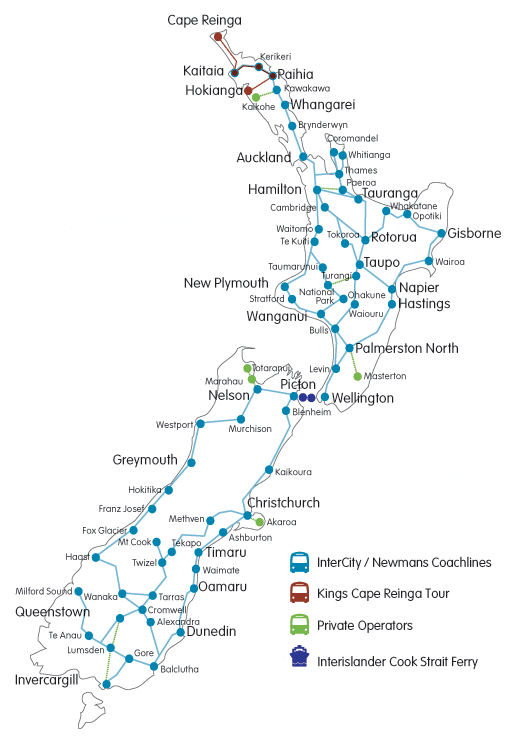
\includegraphics[width=0.75\linewidth]{map.png}
\end{figure}

\footnotesize{\bf{Finding answers:}}
\begin{itemize}
\scriptsize{
\item Inform with transportation data.
\item Simulate forward-time outbreak.}
\end{itemize}
\vspace{3mm}
\end{columns}

\end{frame}
%----------------------------------------------------------------------------------------
\begin{frame}

\begin{columns}[c] % The "c" option specifies centered vertical alignment while the "t" option is used for top vertical alignment

\column{.35\textwidth} 



\column{.65\textwidth} 

%\vspace{5mm}
\begin{figure}
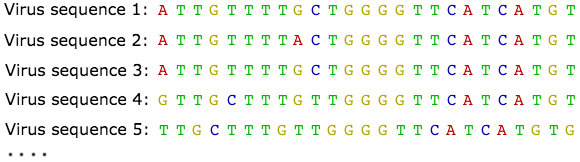
\includegraphics[width=0.9\linewidth]{FluSequence0.png}
\end{figure}
\begin{figure}
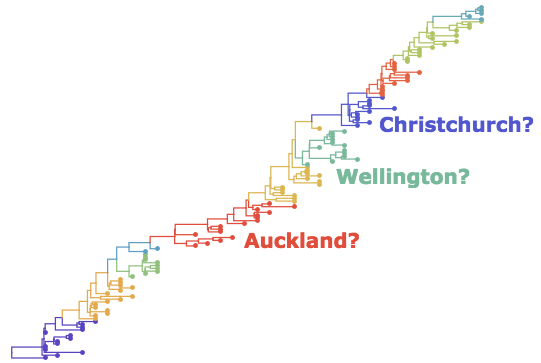
\includegraphics[width=0.9\linewidth]{InfluenzaTree0.png}
\end{figure}
\end{columns}

\end{frame}
%----------------------------------------------------------------------------------------
\end{document} 
